\section{Background and Motivation}
\label{sec:background}

In this section we outline the process for defining a UML profile and supporting model editing facilities in Papyrus. This process consists the manual creation of several interwoven models and configuration files. We highlight labour-intensive and error prone activities involved in the process that motivate the need of automatic generation of those artefacts.

\subsection{UML Profile}
A UML Profile in Papyrus is an EMF model that conforms to the UML Ecore 
metamodel. Thus, in order to create a new UML Profile, developers need to 
create a new UML model and add new elements of type \textit{Stereotype, 
Property, Association, etc.} to create the desired stereotypes, their 
properties and their relationships. Papyrus offers, among other choices, that 
of creating the UML profile via a \textit{Profile Diagram}. Users can 
drag-and-drop elements from the palette to 
construct the profile. The properties of each element (e.g., data types of 
properties, multiplicity, navigability, etc.) can be then set using the 
properties view. In a profile, each stereotype needs to 
extend a UML concept (hereby referred to as \textit{base element} or \textit{meta-element}). Thus, users also need to import these meta-elements and add the 
appropriate extension links with the stereotypes. The process of creating the 
profile can be repetitive and labour-intensive, depending on the size of the 
profile.  
Having created a profile, users can then apply it on a UML model and 
create instances of the stereotypes by applying them to instances of their base 
elements. For example, if a stereotype extends the ``Class'' meta-element in 
UML, users can apply it to selected classes in the model. 

One of the limitations of UML Profiles in Papyrus is that links between 
stereotypes can be instantiated as edges in a diagram only if they  extend a 
\textit{Connector} meta-element (e.g., Association, etc.).  For 
example, if ``Stereotype A'' refers to ``Stereotype B'' via an ``A\_to\_B'' 
reference then in order to be able to draw this connection as an edge on 
the diagram, ``A\_to\_B'' should be created as a separate stereotype. These 
connector stereotypes do not hold any information about the stereotypes that 
they can connect, so users need to define such restrictions by manually writing 
OCL constraints to validate if the source and target nodes are of the desired 
type and if the navigation of the edges is in the correct direction. These 
constraints can be rather long and need to be manually written and customised 
for \textit{each} edge stereotype. This can also be a labour-intensive and 
error-prone process.

\subsection{Distributable Custom Graphical Editor}

At this point, the created profile can be applied on UML 
diagrams. Users select a UML element (e.g., Class) and manually apply the stereotype. A stereotype can only be applied to the UML element that was defined as its 
base element. For example, a stereotype that 
extends the ``Package'' UML meta-class in the profile cannot be applied to a 
``Class'' element. This task might be problematic as users need to remember the 
base elements for each domain-specific stereotype. 
%It is even more 
%problematic in scenarios where the profile was created by someone else. In 
%fact, except from using the profile in their local machine, users can 
%distribute it (all the needed information are stored in a file called 
%``model.profile.uml'') so it can be used by others. 

% Although the aforementioned manual creation and use of the profile sometimes covers all the needs of the stakeholders and includes trade-offs they are willing to take, it is usually the case that stakeholders require the definition of custom shapes for the stereotypes and/or a custom palette of stereotypes. The later is important if one thinks that in smaller profiles, users actually need to navigate through tenths of elements available in the default palette, to pick the one that should be used and apply the stereotype. 

To address this recurring concern, Papyrus offers at least three possible 
options for creating a custom palette which allows users to create base UML 
elements and apply selected stereotypes on them in a single step. The first 
option involves customisation through a user interface where users add elements 
in the palette for their stereotypes. Although this is an 
easy-to-use approach, it has to be done manually when a new diagram is created 
while it cannot be shared in case the profile needs to be distributed with 
collaborators. 

The other two options require the manual definition of palette configuration 
files that are automatically loaded every time the profile is applied on a 
diagram. Although the first is simpler and requires the definition of a single 
XML file, it is not encouraged as it does not allow the full use of Papyrus 
functionality. Furthermore, this option is based on a deprecated framework, and 
its use is not encouraged.

%While the first is simpler and requires the definition of one XML file, is not 
%encouraged as it does not allow the full use of Papyrus functionality while it 
%is deprecated in the latest versions of the tool.

The definition of custom shapes for the instantiated stereotypes is another 
common requirement. Scalable Vector Graphics (SVG) shapes can be bound to 
stereotypes at the profile creation process. However, to make these shapes  
visible, users need set the visibility of the shape of \textit{each} element to true. Even if this is an 
acceptable trade-off, another drawback is that by default the shape overlaps 
with the default shape of the base meta-element. Users can hide the default 
shapes by writing CSS rules. The rules can 
be written once but need to be loaded each time \textit{manually} on every 
diagram that is created. 

\begin{figure}[t]
	\centering
	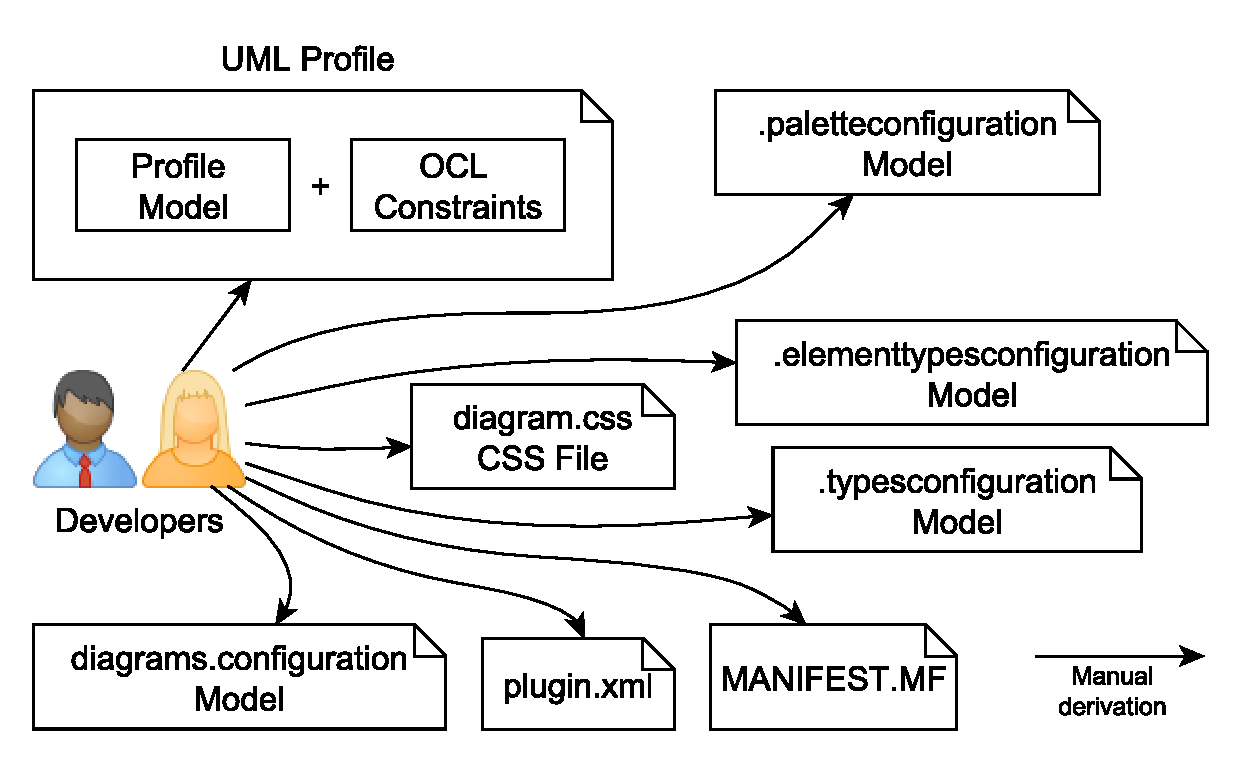
\includegraphics[width=1\textwidth]{diagrams/neededPapyrusFiles.pdf}
	\vspace{-3mm}
	\caption[]{All the models/files developers need to write manually to 
	develop a fully functional distributable Papyrus profile and editor plugin.}
	\label{fig:neededPapyrusFiles}
	\vspace*{-3mm}
\end{figure}

To create a distributable graphical editor that has diagrams tailored for the 
profile and to avoid all the aforementioned drawbacks, users need to create 
several models and files and add extensions pointing to them in a plugin 
project. Figure~\ref{fig:neededPapyrusFiles} shows all the files needed to be 
created \textit{manually} for having a distributable Papyrus plugin 
graphical editor. This plugin has a custom palette for the profile, can 
automatically assign stereotypes to the elements and can automatically 
apply a CSS stylesheet to the diagrams. 
An explanation of each file is provided in Section~\ref{sec:implementation}. A 
few hundred lines of code need to be written while tedious plugin creation and 
repetitive model creation tasks should be done. 


This \textit{labour-intensive}, \textit{repetitive} and \textit{error-prone} 
process could be automated. In this work, we propose an approach that uses a 
single-source input to automatically generate the UML profile and all the 
models/files mentioned above. This 
approach is described in Section~\ref{sec:approach} that follows. 
